\subsection{Very Forward Detectors}
%\writer{Yan Benhammou, Sergej Schuwalow}{2}

In the past years the development of the ILD forward detectors has mostly been pursued by the FCAL R\&D Collaboration~\cite{ild:bib:FCAL}. Progress concerns mainly the LumiCAL calorimeter and, more recently, the BeamCAL sensors.

Based on a specific ASIC developed after the DBD, calorimeter silicon sensitive layers have been built to assemble a first LumiCAL 4-layer tungsten calorimeter prototype and, two years later, a more compact 8-layer calorimeter prototype (Figure~\ref{fig:det:LUMICAL_perf} left). The two prototypes were tested with beam in 2014 and 2016, respectively. The test data~\cite{Abramowicz:2018vwb} confirm the expected significant improvement of the transverse compactness of the electromagnetic showers in the compact prototype compared to the earlier one (Figure~\ref{fig:det:LUMICAL_perf} right). 

A new ASIC "FLAME"~\cite{ild:bib:FLAME} based on 130 nm CMOS technology is currently under final validation. FLAME features the low power, in-situ digitisation and fast readout required by the final detector. A new $\approx$20- layer SiW calorimeter prototype based on FLAME, with specifications and configuration close to the final LumiCAL detector, is under construction and planned to be tested with beam in 2019. 

\begin{figure}[t!]
\centering
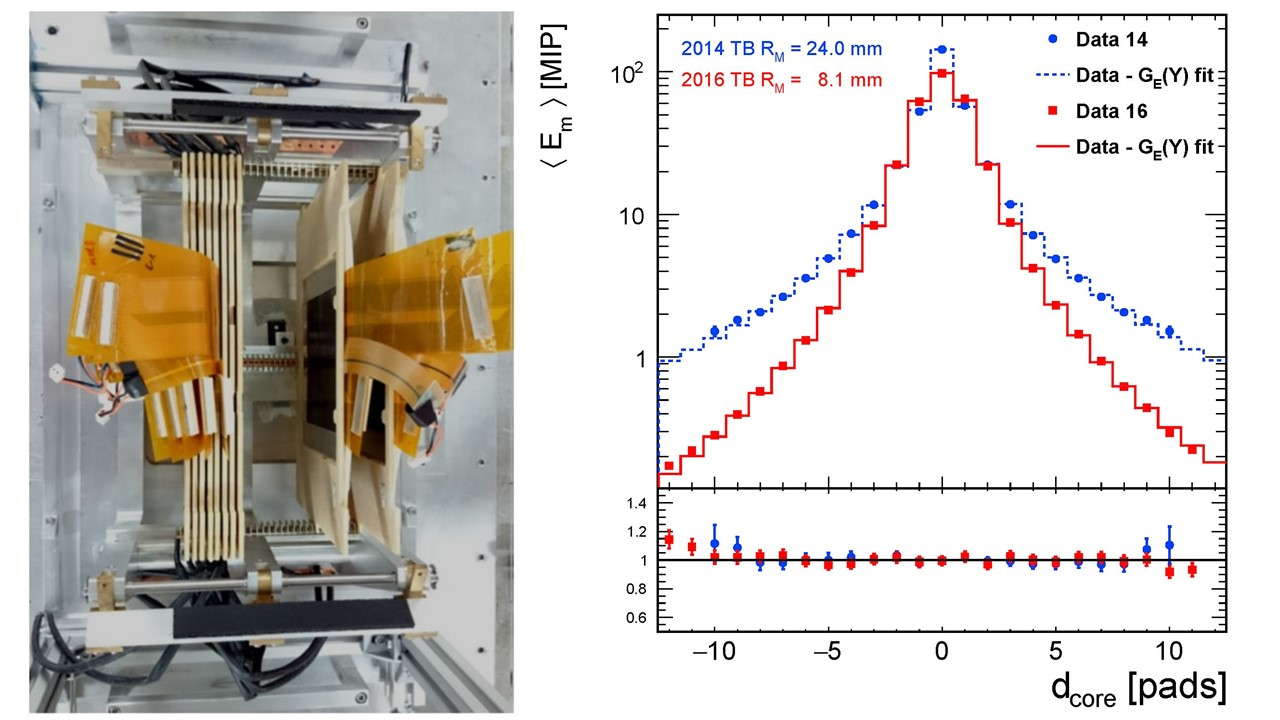
\includegraphics[width=1.0\hsize]{Detector/fig/LUMICAL_perf.jpg}
\caption{LumiCAL compact prototype tested in the DESY electron beam in 2016 (left) and corresponding improvement in shower compactness achieved versus the 2014 prototype (right).}
\label{fig:det:LUMICAL_perf}
\end{figure}

The LHCAL and BeamCAL calorimeters can be based on similar technologies as the LumiCAL, with radiation hardness requirements increasing as function of the sensor proximity to the beam. For the BeamCAL, new sensors such as sapphire are being considered. Irradiation campaigns are under way to characterize them (Figure~\ref{fig:det:BEAMCAL_rad}) and provide input for the final choice. 

\begin{figure}[t!]
\centering
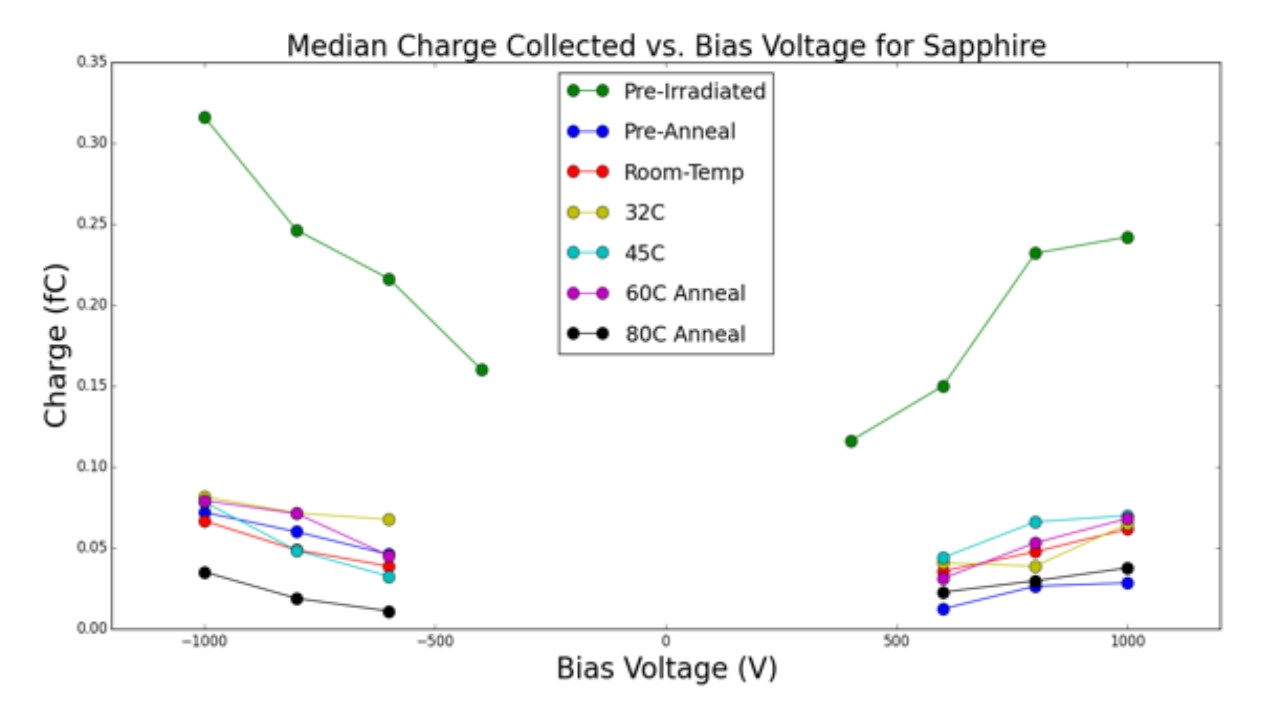
\includegraphics[width=0.8\hsize]{Detector/fig/BEAMCAL_rad.jpg}
\caption{results of irradiation tests performed at SLAC for sapphire sensors considered for the BeamCAL.}
\label{fig:det:BEAMCAL_rad}
\end{figure}